%% ****** Start of file apstemplate.tex ****** %
%%
%%
%%   This file is part of the APS files in the REVTeX 4 distribution.
%%   Version 4.1r of REVTeX, August 2010
%%
%%
%%   Copyright (c) 2001, 2009, 2010 The American Physical Society.
%%
%%   See the REVTeX 4 README file for restrictions and more information.
%%
%
% This is a template for producing manuscripts for use with REVTEX 4.0
% Copy this file to another name and then work on that file.
% That way, you always have this original template file to use.
%
% Group addresses by affiliation; use superscriptaddress for long
% author lists, or if there are many overlapping affiliations.
% For Phys. Rev. appearance, change preprint to twocolumn.
% Choose pra, prb, prc, prd, pre, prl, prstab, prstper, or rmp for journal
%  Add 'draft' option to mark overfull boxes with black boxes
%  Add 'showpacs' option to make PACS codes appear
%  Add 'showkeys' option to make keywords appear
%\documentclass[aps,prl,preprint,groupedaddress]{revtex4-1}
%\documentclass[aps,prl,preprint,superscriptaddress]{revtex4-1}
\documentclass[aps,pra,reprint,superscriptaddress]{revtex4-1}

% You should use BibTeX and apsrev.bst for references
% Choosing a journal automatically selects the correct APS
% BibTeX style file (bst file), so only uncomment the line
% below if necessary.
%\bibliographystyle{apsrev4-1}
\usepackage[utf8]{inputenc} % Danish characters
\usepackage{graphicx}% Include figure files
\usepackage{dcolumn}% Align table columns on decimal point
\usepackage{clrscode}
\usepackage{bm}% bold math
\usepackage{xcolor}
\usepackage{amsmath}
\usepackage{hyperref}
\usepackage{braket}
\usepackage{bbold}
\usepackage{verbatim}
\usepackage{caption}
\usepackage{subcaption}

%% Tikz stuff
\usepackage{tikz}
\usetikzlibrary{shapes.geometric, arrows}

% Tikz shapes
\tikzstyle{component} = [rectangle, rounded corners, minimum width=1cm, minimum height=1cm, text centered, draw=black, fill=red!30]
\tikzstyle{input} = [rectangle, rounded corners, minimum width=1cm, minimum height=1cm, text centered, draw=black, fill=green!30]


\begin{document}

% Use the \preprint command to place your local institutional report
% number in the upper righthand corner of the title page in preprint mode.
% Multiple \preprint commands are allowed.
% Use the 'preprintnumbers' class option to override journal defaults
% to display numbers if necessary
%\preprint{}

%Title of paper
\title{Quantum Control report}

% repeat the \author .. \affiliation  etc. as needed
% \email, \thanks, \homepage, \altaffiliation all apply to the current
% author. Explanatory text should go in the []'s, actual e-mail
% address or url should go in the {}'s for \email and \homepage.
% Please use the appropriate macro foreach each type of information

% \affiliation command applies to all authors since the last
% \affiliation command. The \affiliation command should follow the
% other information
% \affiliation can be followed by \email, \homepage, \thanks as well.
\author{Tobias Rasmussen}
\affiliation{Department of Physics and Astronomy, Aarhus University, Ny Munkegade 120, 8000 Aarhus C, Denmark}
\email{201608265@post.au.dk}
%\homepage[]{Your web page}
%\thanks{}
%\altaffiliation{}


%Collaboration name if desired (requires use of superscriptaddress
%option in \documentclass). \noaffiliation is required (may also be
%used with the \author command).
%\collaboration can be followed by \email, \homepage, \thanks as well.
%\collaboration{}
%\noaffiliation

\date{\today}

%\begin{abstract}
% insert abstract here
%{This is a very preliminary document describing the efforts regarding implementation of spintronic systems in the Aarhus University quantum gas microscope.}
%\end{abstract}

% insert suggested PACS numbers in braces on next line
%\pacs{37.25.+k,37.10.Jk, 03.75.Dg}
% insert suggested keywords - APS authors don't need to do this
%\keywords{}

%\maketitle must follow title, authors, abstract, \pacs, and \keywords
\maketitle

% body of paper here - Use proper section commands

\section{Introduction}
%Here, you should write an introduction that describes what specific problems you explored. Your introduction should also describe how the document is structured (e.g. ``Section \ref{sec:back} describes how I invented underwater basket weaving for Bose-Einstein condensates...''). You should also briefly describe the main results, but keep this to a sentence or two. The rest of the report should elaborate on those results and the methods you used to find them.
In the Shake Up challenge, one works with a state confined in a trapping potential. The state describes either a single particle or a Bose Einstein Condensate (BEC) state of matter and starts in the ground state of the given potential. The goal is now to translate the potential in such a way that the state is completely excited from its ground state to its first excited state. The potential is moved using a control function $u(t)$, which in this challenge can be either an analytical function or created by dragging points on a discretized line. The problem is simulated and exploted using the software Quantum Composer. One uses the fidelity $F = | \langle \phi | \psi \rangle |^2$ to calculate how much of the state $\ket{\psi}$ 'is in' the desired state $\ket{\phi}$ and so as a measure for how well a given control function performed.\\

Furthermore, the self picked goal of the challenge was to explore the different dynamics that arise when simulating the BEC compared to a single particle, how these dynamics depend on the nonlinearity of the BEC Hamiltonian and how this nonlinearity affects the Quantum Speed Limit (QSL). Adding to this is exploring how controls can be clustered, how optimal solutions look compared to similar ones and how robust they are to changes to the system.\\

This report is structured as follows: In section \ref{sec:back} some background information regarding the challenge is provided. Section \ref{sec:results} contains the results of the report and is split into 3 parts. Section \ref{subsec:obs} shows the results of exploring this challenge by simulating BECs in a number of different systems, section \ref{subsec:strats} explains the strategies used to reach those results and \ref{subsec:numericalLimitations} discuss some of the limitations to exploring the problem using Quantum Composer that were found. The results are then discussed in section \ref{sec:disc}.

In section \ref{sec:conclusion} it is concluded that the nonlinear term for the BEC drastically changes the behavior of the state compared to the single particle state for values of $\beta$. This new behavior could, in some cases, improve the reachable fidelity compared to a single particle by up to $50\%$. It was also found that the value of $\beta$ affects the QSL of BECs. This section also sums up the conclusions about the different approaches to creating a control function that were used in this project. Finally, a number of things for future study of the subject are suggested.

\section{\label{sec:back}Background}
%Here, you can describe the background of your problem. What motivated you to explore this particular problem? Describe your general strategy. What do we need to know to understand your results?
The Hamiltonian describing a single particle in a trapped, controlled potential takes the form:
\begin{equation}
	H(x,t) = \frac{p^2}{2m} + V(x,u(t))
\end{equation}
where $p$ is the momentum operator and $m$ is the particle mass. Likewise, the Hamiltonian of a BEC can be approximated to obey the Gross-Pitaevskii equation
\begin{equation}
	H_{GPE} = \frac{p^2}{2m} + V(x,u(t)) + \beta |\psi(x,t)|^2
	\label{eq:Hbec}
\end{equation}
which contains a nonlinear term with front factor $\beta$ compared to the Hamiltonian for a single particle. This term represents the interatomic interaction that takes place in a BEC. This factor is both dependent on the s-wave scattering length $a_{\text{1D}}^s$ as well as the number of atoms contained in the BEC $N$ \cite{Schmiedmayer}. It is however, also possible to tune this interaction parameter using Feshbach a resonance \cite{Feshbach}.


The problem was explored by adjusting $\beta$, the control final time $T$, the control function $u(t)$ as well as working with different trapping potentials.

Depending on the sign of $\beta$ in \eqref{eq:Hbec} the interatomic interaction will be either attractive ($\beta<0$) or repulsive ($\beta>0$) and based on this, we would expect the state to respectively shrink or grow in size as a result of this interaction. This is also what can be seen on Fig. \ref{fig:BECgroundstate}, where the ground state is plotted as a function of $\beta$.

\begin{figure}[h]
	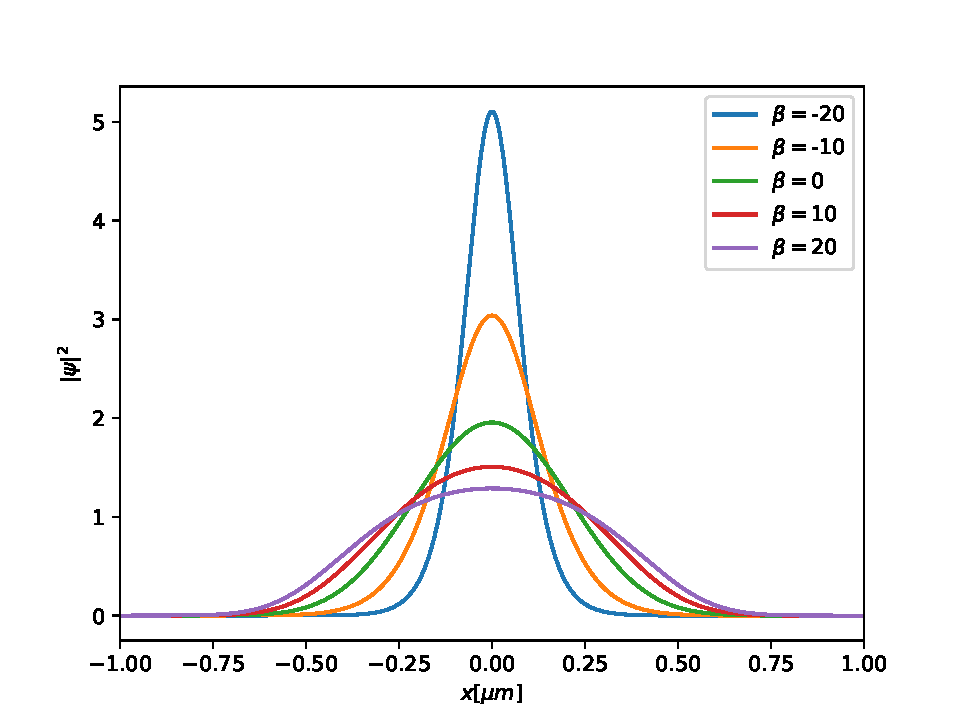
\includegraphics[width=\columnwidth]{graphics/GroundstateBeta.pdf}
	\caption{The groundstate of a BEC in a quartic trapping potential, shown as a function of the atomic interaction parameter $\beta$ in \ref{eq:Hbec}.}
	\label{fig:BECgroundstate}
\end{figure}

The 1st excited state likewise shares this property, but since this state is already larger than the ground state, its size is not altered by $\beta$ to the same extend. This is shown on figure \ref{fig:BECexcitedstate}.

\begin{figure}
	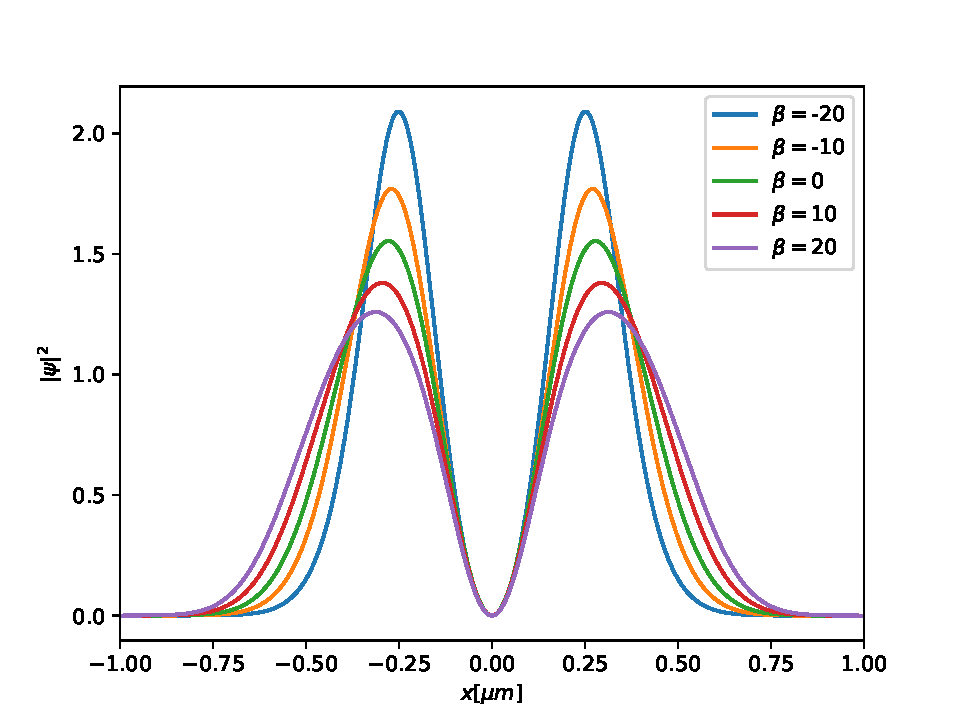
\includegraphics[width=\columnwidth]{graphics/ExcitedstateBeta.pdf}
	\caption{The 1st excited state of a BEC in a quartic trapping potential. This is the desired state which we attempt to transform the initial ground state into.}
	\label{fig:BECexcitedstate}
\end{figure}

It is possible to optimize a control function to, in many cases, reach even higher fidelity than the initial function. In this problem the optimization algorithm $\proc{Grape}$ is used. $\proc{Grape}$ takes an input control function (a "seed"), and calculates the gradient of $F$ with respect to each point of the control function on the discretized time scale $\vec{\nabla}_{\vec{u}}F(\vec{u})$, such that $\vec{u} = (u(t_0), u(t_1) ... \,, u(T))$. When this calculation is done, $\proc{Grape}$ takes a step of size $\alpha_k$ such that the new discretized control function becomes
\begin{equation}
	\vec{u}_{k+1} = \vec{u}_{k} + \alpha_k \vec{\nabla}_{\vec{u}}F(\vec{u}_k)
\end{equation}
where $F(\vec{u}_{k+1}) \geq F(\vec{u}_{k})$.

This process is continued until some convergence criterium is fulfilled, e.g. a target threshold $F(\vec{u}_{k}) \geq F_{target}$ or a maximum number of iterations $k \leq N$.

\section{Quantum Composer}
The plan is here to add Screenshots about how Composer is used in this project.
Also a flowchart describing the workflow would be nice.
Below is a tikzstyle picture
\begin{figure}
	\centering
	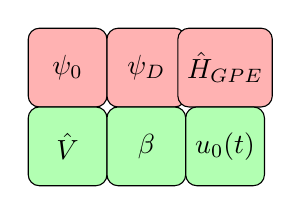
\begin{tikzpicture}
		\node (psi0) [component] {$\psi_0$};
		\node (psiD) [component, right of=psi0] {$\psi_D$};
		\node (H) [component, right of=psiD] {$\hat{H}_{GPE}$};	
		\node (V) [input, below of=psi0] {$\hat{V}$};
		\node (beta) [input, right of=V] {$\beta$};
		\node (u0) [input, right of=beta] {$u_0(t)$};
	\end{tikzpicture}
	\caption{Work flow in Quantum Composer}
	\label{fig:flowdiagram}
\end{figure}


\section{\label{sec:results}Results}
%This should be the bulk of your report. Describe your results. Any details (not included in the background) that are necessary to understand what you did should be here.

%You can include citations with the \verb+\cite{}+ command. You will need a \verb+.bib+ file like the one included with this template. See the bibliography file for information on how to cite an article \cite{Schmiedmayer2014}, a thesis \cite{HenrikThesis}, or a book \cite{PethickSmith}. If you do not include any citations, comment the \verb+\bibliography{}+ command below.
\subsection{\label{subsec:numericalLimitations} Numerical limitations}
In order to reach accurate results when making these computations, one has to ensure that the states that are analyzed are described within acceptable numerical accuracy. We can ensure that we are working with the ground state as our initial state in Composer by calculating the variance of our initial state wrt. the Hamiltonian
\begin{equation}
	\text{Var}(\psi)_H = \langle \psi \mid \hat{H}^2 \mid \psi \rangle - (\langle \psi \mid \hat{H} \mid \psi \rangle)^2
\end{equation}

This gives us a numerical estimate of how "close" our initial state is to the actual ground state of $\hat{H}_{GPE}$ since
\begin{equation}
	\psi \text{ is an eigenstate of } \hat{H}_{GPE} \iff \textsc{Var}(\psi)_H = 0
\end{equation}

The way the energy spectrum of $\hat{H}_{GPE}$ is calculated is not trivial \cite{QEngine}, but the variance can generally be reduced by adjusting different parameters of the system or Composer file, e.g. spatial dimension $x$ or initial conditions for the $H_{GPE}$ spectrum node. Despite these possible fixes, the numerical limitations of Quantum Composer become apparent as the "Shake Up" problem is explored in increasingly greater details and limits and accuracy are pushed further and further. The following paragraphs describe areas where the numerical limitations are significantly limiting the exploration of certain aspects of this problem.\\

As the work with the QSL shown in figure \ref{fig:QSL} was explored, it was desirable to examine how the energy levels of the state changed as a function of $\beta$. The idea was that $\beta$ could change the spacing between the different levels of the potential well and perhaps make the spacing more even for some high or low values of $\beta$. As was shown in figure \ref{fig:HO}, the even spacing of a harmonic quadratic potential makes it difficult to reach the high fidelities desired. To investigate this, the energy difference between the first excited state and the ground state as well as the difference between the second and first excited state was calculated in Composer. The calculated differences are shown in figure \ref{fig:energyDiff} and show that the uncertainty of the second excited state energy rapidly increases as $\beta$ moves away from $0$. It since became apparent that it is not possible to calculate the second excited state of a BEC in Quantum Composer \cite{QEngine}. This nonetheless represents a numerical limitation to exploring this problem. \\

\begin{figure}
	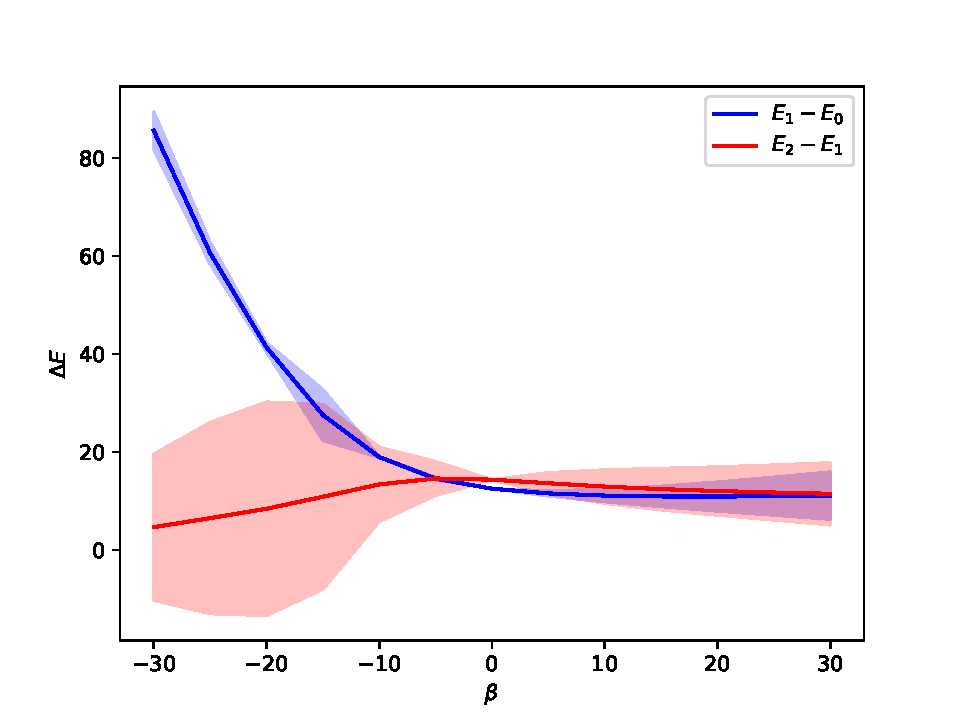
\includegraphics[width=\columnwidth]{graphics/Energydifference.pdf}
	\caption{Energy difference between the first 3 excited states of a BEC in a quartic potential. Note that it is not possible to calculate the second excited state of a BEC in Quantum Composer, and so these values are not valid.}
	\label{fig:energyDiff}
\end{figure}

Despite not being able to calculate the second excited state of a BEC, it was also desired to explore how the ground and first excited state energies changed as a function of $\beta$. These energies are plotted on figure \ref{fig:energyLevels} and as can be seen, the uncertainty regarding the first excited state increases for values of $\beta$ below $-10$. As mentioned when estimating the optimizable limit of negative $\beta$'s, this could explain why $\beta=-10$ is the optimizable limit found.\\

\begin{figure}
	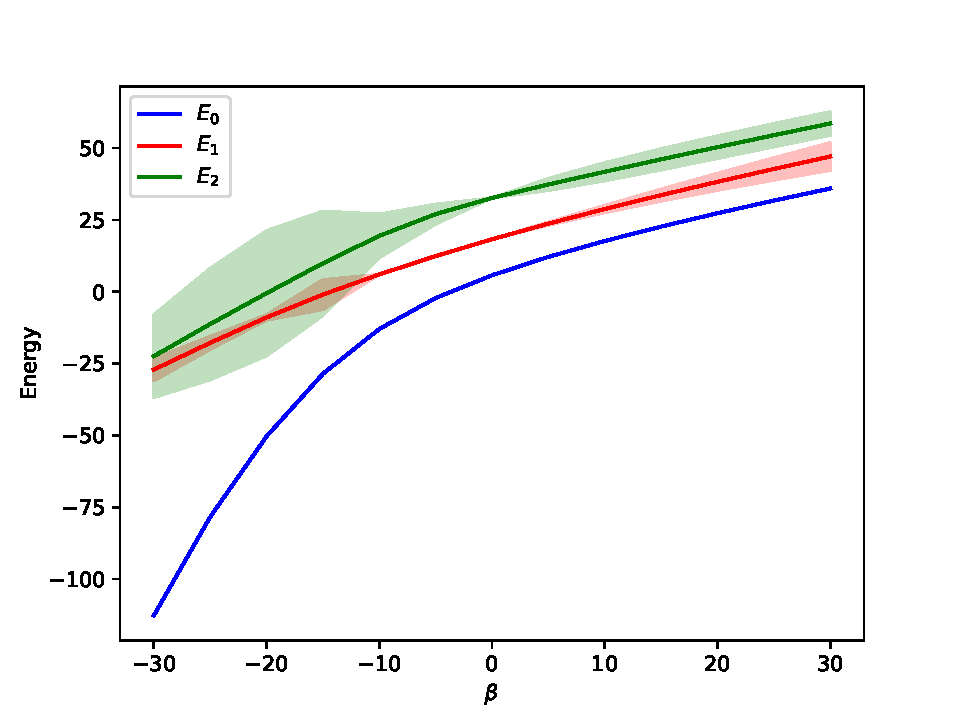
\includegraphics[width=\columnwidth]{graphics/Energylevels.pdf}
	\caption{Calculated energies of the ground and first excited state of a BEC in a quartic potential as a function of $\beta$.}
	\label{fig:energyLevels}
\end{figure}

Even when working within the low-variance range of this problem, one still has to be careful of numerical errors caused by the control function used. These problems with the control function seem to be caused by a combination of different factors: 1. Using 'high' frequency control functions. 2. Initial control functions having large displacements. 3. Larger control durations. As an example, one can see how the $k=4$ seed from figure \ref{fig:Clustering} performed for a duration of $T\approx 0.85$ms compared to a $k=5$ with longer duration  $T\approx 1.0$ms with a smaller amplitude. The comparison can be seen in figure \ref{fig:statePlots} where the resulting state evolution of each of these optimized seeds are shown. The consequence of this error is that the control space that is possible to explore in Composer is limited to what can be handled without breaking the state due to inaccuracy. Thus, high frequency controls can be explored, but if sufficiently large durations are desired, then the amplitude of this oscillation must be scaled to accommodate this.

\begin{figure}
	\begin{subfigure}{0.45\columnwidth}
		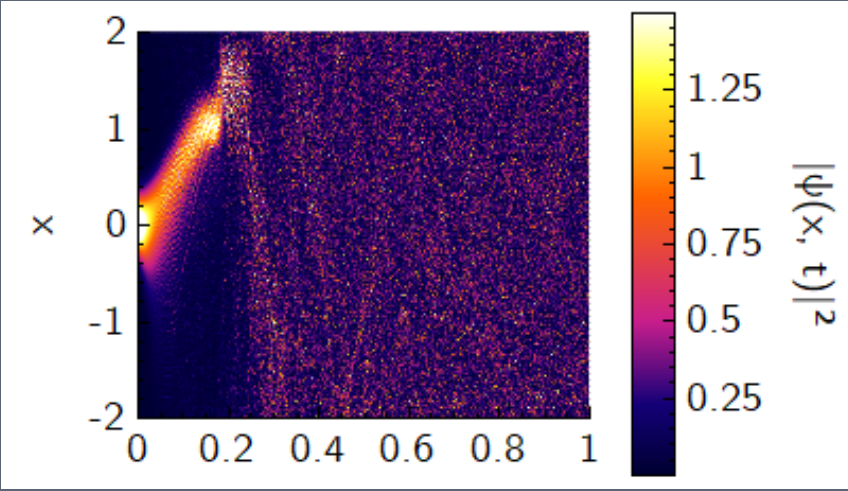
\includegraphics[width=\columnwidth]{graphics/newclustering/QM2Clusteringk4A04T06178-2.PNG}
	\end{subfigure}
	\begin{subfigure}{0.45\columnwidth}
		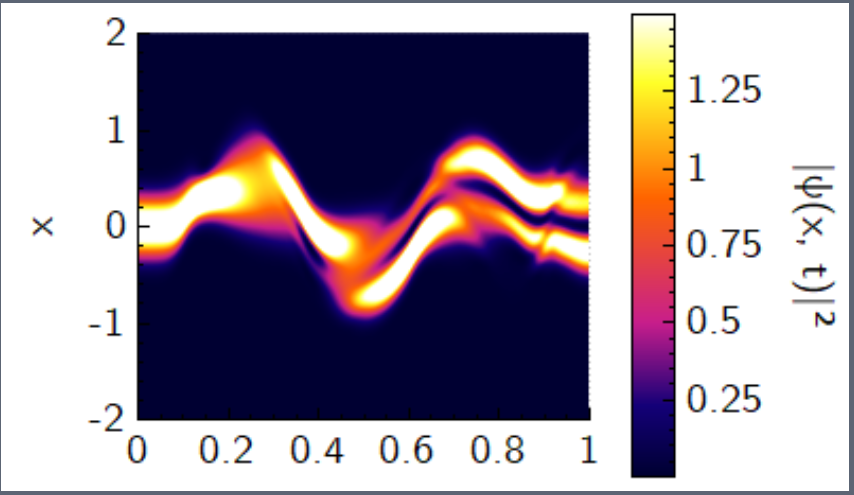
\includegraphics[width=\columnwidth]{graphics/newclustering/QM2Clusteringk5A015T07475-2.PNG}
	\end{subfigure}
	\caption{Comparison of the state evolution for a numerically broken state (left) and a numerically working state (right). On the first axis is normalized control time and on the second axis position in $\mu$m.}
	\label{fig:statePlots}
\end{figure}

\subsection{\label{subsec:obs}Challenge exploration}
% Single particle
Single particles are simple to control. In a quartic potential one can write up many simple control functions which are all able to reach $F\approx0.99$ after at most 25 iterations of $\proc{Grape}$. This is not the case in the quadratic potential since the state is easily excited beyond the desired state due to the equal spacing of energy eigenstates. \\

% BEC in anharmonic
Through simulations it seems that BECs have very different dynamics compared to single particles. Without using $\proc{Grape}$, one can study how the similarity between single particles and BECs changes depending on the value of $\beta$. Keeping the control function and control duration the same, we find that what was a good solution for a single particle reaches a lower and lower fidelity as we change $\beta$ away from 0, but that it also reaches revivals with a higher fidelity compared to neighboring values. This behavior is shown in figure \ref{fig:beta} where the non-optimized control
\begin{equation}
	u_{\mathrm{non-opt}}(t)=0.12\cdot\sin(0.86\cdot \omega_{01} t)
\end{equation} with final time $T=3.49$ was simulated for different values of $\beta$. We define $\omega_{01}$ to be the energy frequency between the ground and first excited state.

\begin{figure}[h]
	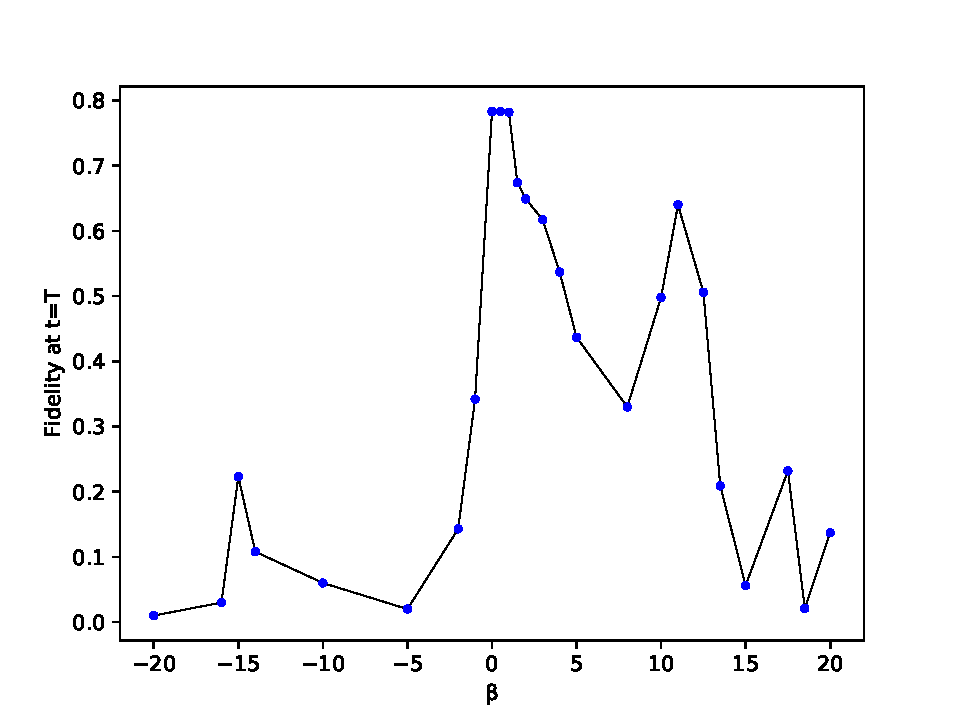
\includegraphics[width=\columnwidth]{graphics/beta.pdf}
	\caption{Fidelity of a non-optimized solution for different values of $\beta$ in a quartic potential.}
	\label{fig:beta}
\end{figure}

% For large T we observe different behavior for BECs and SPs
When studying BECs in the quartic potential, it was found that for small $\beta<5$ it was possible to optimize the state to reach the same high fidelity as for the single particle case. For larger values of $\beta$, it was observed that the final fidelity converged on increasingly smaller values. The fidelity could be improved by raising/lowering the final time $T$, but for large $\beta > 25$ the maximum reachable fidelity with $\proc{Grape}$ decreases to below $0.99$. So obviously there exists some relationship between $\beta$ and $T$ where some combinations result in high fidelity while others do not. This could also explain why some values of $\beta$ in figure \ref{fig:beta} increase the fidelity in a small region (e.g. around $\beta=10$) as if there is some kind of resonance. \\

% BEC in harmonic
The nonlinear interaction term of the BEC Hamiltonian also had a positive effect when optimizing BECs in the harmonic potential case. Here, this term caused a greater final fidelity for some values of $\beta$ than in the single particle case, where it was difficult to reach a fidelity of $0.4$. This is shown in figure \ref{fig:HO}.\\
%TODO This might be due to numerical inacc
\begin{figure}[h]
	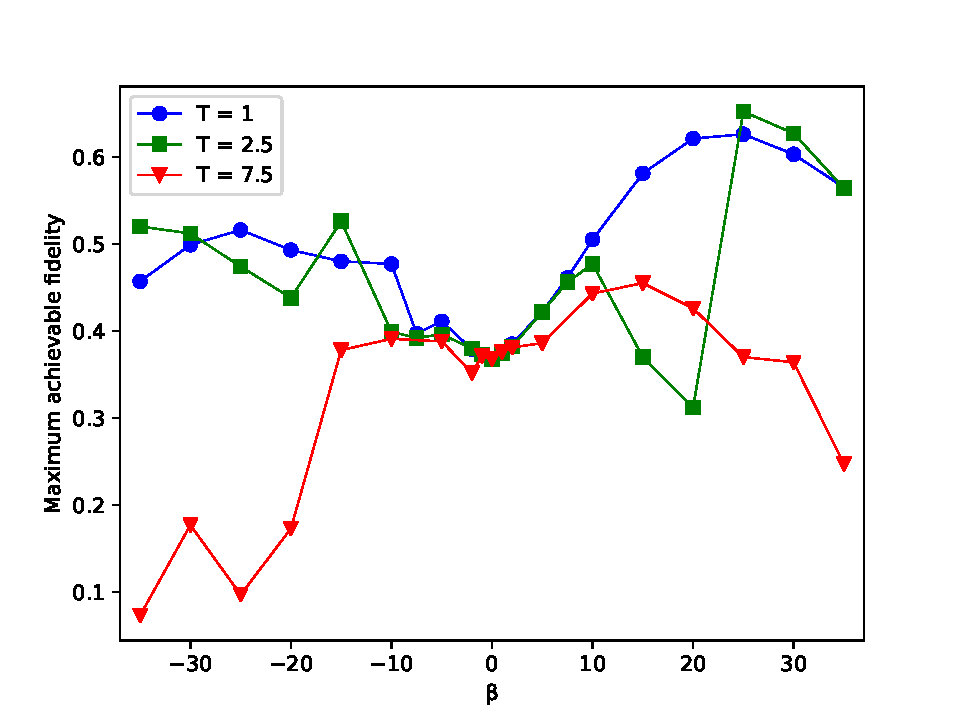
\includegraphics[width=\columnwidth]{graphics/betaTHO.pdf}
	\caption{The result of varying $\beta$ and $T$ for a BEC in the harmonic potential. As it can be seen, there exists 'resonant' combinations where it is possible to achieve above $50\%$ higher fidelity compared to a single particle (at $\beta=0$), but many also combinations that are on par with or worse than a single particle.}
	\label{fig:HO}
\end{figure}

%QSL
Studying the Quantum Speed Limit for this problem yields the results shown on figure \ref{fig:QSL}. The figure shows how different values of $\beta$ impacts the QSL for BECs in the anharmonic potential. As it can be seen, $\beta$ values away from 0 raise the speed limit increasingly the further away from 0 they are. \\

\begin{figure}[h]
	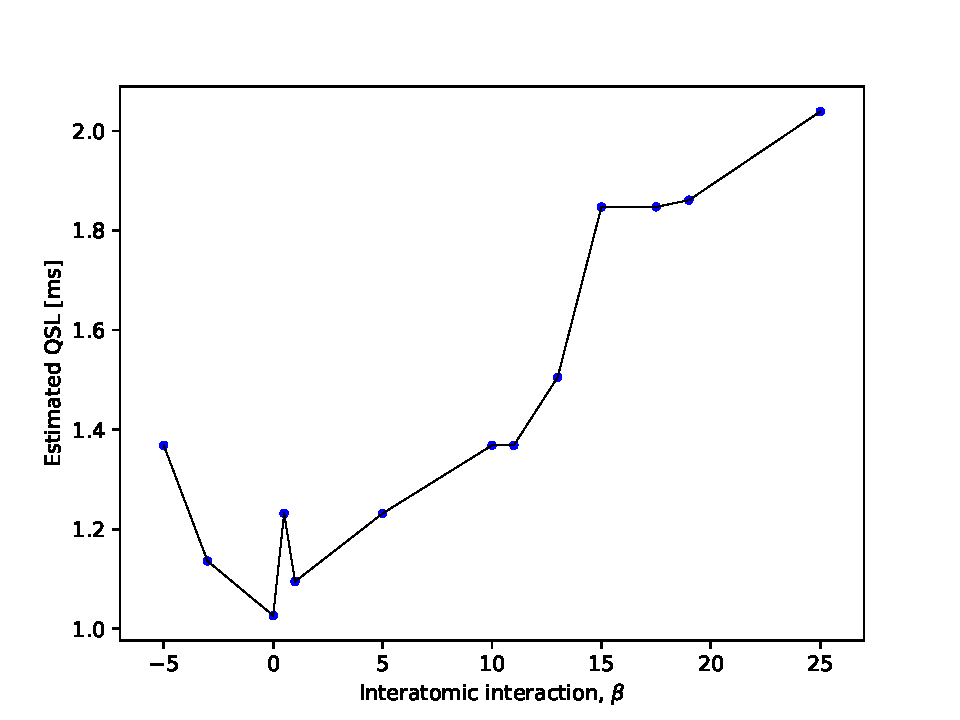
\includegraphics[width=\columnwidth]{graphics/QSL.pdf}
	\caption{The estimated Quantum Speed Limit for a BEC in the anharmonic potential as a function of $\beta$. The behavior of the BEC at $\beta=0$ is the same as for a single particle. Notice how the QSL is doubled compared to a single particle when $\beta=25$. It has not been possible to reach the required fidelity for any $\beta < 5$.}
	\label{fig:QSL}
\end{figure}

It is clear after having explored the behavior of BECs in different numerical setups that the behavior the BECs are not symmetric with respect to $\beta$. This is not unexpected, since the sign of $\beta$ constitutes whether the atom-atom interaction happening inside the BEC is repulsive($\beta>0$) or attractive ($\beta<0$) and so it would not be unjustified to say that the sign of $\beta$ describe entirely different species of bosons. Since attractive BECs have proven difficult to optimize on for $\beta<-5$, it was explored what the lower limit of $\beta$ would be with respect to reaching an optimizable fidelity of at least $0.99$. The results of this exploration is seen on figure \ref{fig:reachable_neg_betas}, where it can be seen that for values of $\beta<-10$ it is no longer possible to reach $F~0.99$. In subsection \ref{subsec:numericalLimitations}, this observation is discussed.

%TODO Mention what red line is
\begin{figure}
	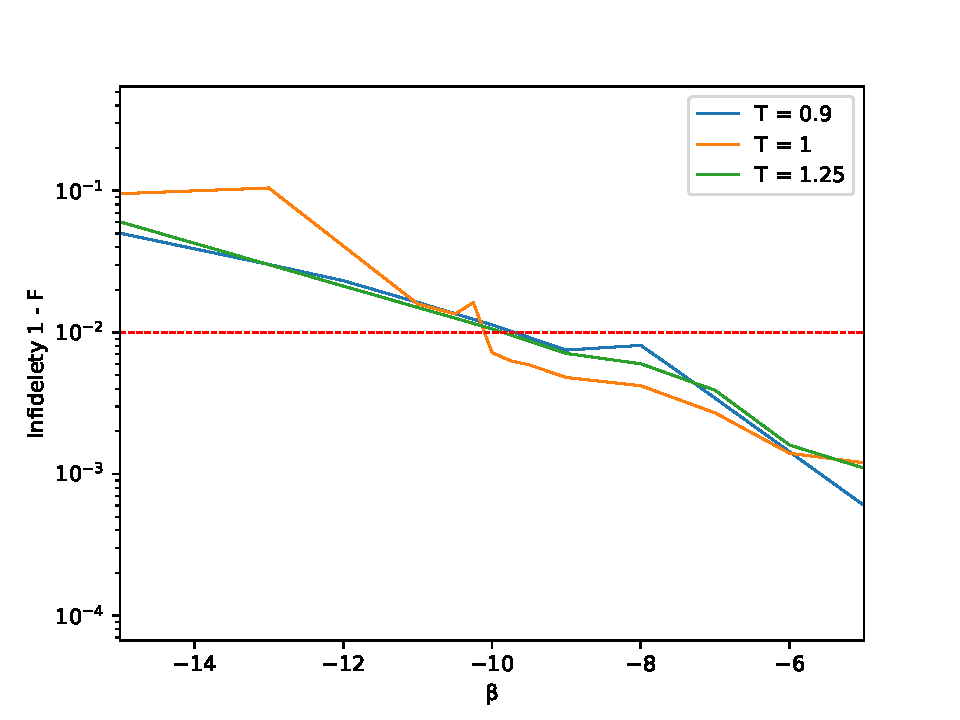
\includegraphics[width=\columnwidth]{graphics/reachable_neg_beta.pdf}
	\caption{Lowest reachable infidelities as a function of interatomic attraction $\beta$, shown for different timescales. It seems that $\beta=-10$ is the lower limit for reaching optimizable solutions $F~0.99$. This lower limit is, however, suspected to be caused by numerical inaccuracies.}
	\label{fig:reachable_neg_betas}
\end{figure}

%clustering of solutions
\subsection{\label{subsec:clustering}Clustering of solutions}
In a recent article where this problem has also been studied \cite{QM2Paper}, it was found that optimal solutions for increasing final times were dominated by cosine functions of increasing frequencies $k\pi t/T$. It was attempted to replicate this result by letting \proc{Grape} optimize seeds on the form $u(t) = A\cos(k\pi t/T)$ for 750 iterations each. By varying $k$ and $A$, the frequency and amplitude of the seeds were varied and their optimized solutions and reached fidelity noted. The results can be seen on figure \ref{fig:Clustering}. As can be seen on the figure, the results do not replicate those found in \cite{QM2Paper} where solutions dominated by different values of $k$ outperform other $k$'s for some interval. Note in particular that the overall highest fidelity was reached for a seed with frequency $k=2$ at $ T\approx 0.93 \text{ms} $, where $ k=5 $ was expected to be the best performing frequency. However, note that both $k=4$ and $k=5$ reach solutions that outperform the other seeds for that particular timescale and that they do so in the expected order (4 before 5). It should also be mentioned that the $k=4$ data span a smaller time interval due to numerical errors in their solutions for $T>0.8 ms$. This is discussed further in section \ref{subsec:numericalLimitations}. \\

To replicate the results found in \cite{QM2Paper}, the system conditions had to be replicated in Composer where the scales are chosen from the requirement $\hbar = m = 1 \Rightarrow \chi = 1\mu m, \, \tau \approx 1.36$ where $\chi$ and $\tau$ are the scales of length and time respectively, such that $x_{SI}=\chi x$ etc. The paper has on the other hand chosen scales such that $\chi = 1 \mu\text{m}$ and $\tau = 1 \text{ms}$ \cite{QEngine}. This results in a conversion factor of $\kappa = 1.36537$ compared to those found in \cite{QEngine} of the following quantities: $\beta_{old} = 1.8299 \rightarrow \beta = 2.5042 = \kappa \beta_{old}$, $p_i \rightarrow \kappa p_i$ where $V(x,u(t)) = \sum_{i=2,4,6} p_i (x-u(t))^i$ is the potential of the system and finally $\tau$. \\

\begin{figure}
	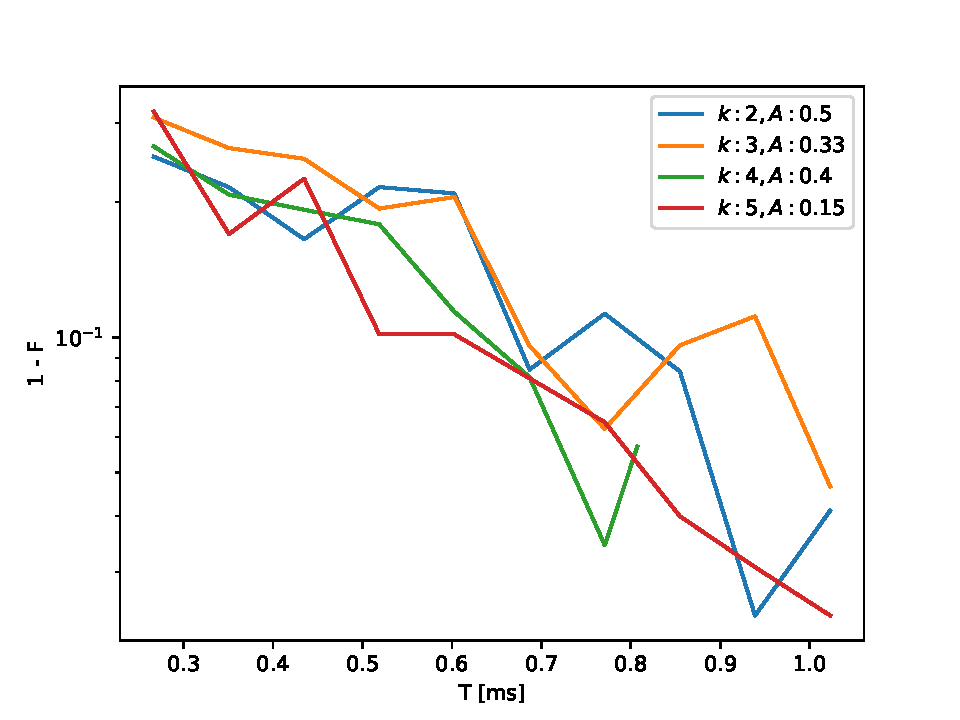
\includegraphics[width=\columnwidth]{graphics/newclustering/QM2Clustering.pdf}
	\caption{Infidelity of \proc{Grape} optimized solutions with initial control $u(t)=A\cos(k\pi t/T)$. The first axis shows the control duration $T$.}
	\label{fig:Clustering}
\end{figure}

\subsection{\label{subsec:robustness} Robustness of solutions}
The robustness of optimized solutions wrt. interaction strength or potential scaling was studied in \cite{GroupPaper}. This is interesting since real experiments are often subject to the inherent uncertainties of their equipment e.g. the frequency width of a laser. Since the interatomic interaction in a BEC is dependent on the number of atoms it consists of, it is not surprising that a specific factor $\beta$ is difficult to replicate exactly in the lab. Likewise the trapping potential is created by standing waves of laser light and so it is also subject to some uncertainty in intensity and frequency.  \\

The robustness of optimized solutions was replicated for the same system as the solution clustering. This replication was done by letting \proc{Grape} optimize the same control seed, $u(t)=0.15\cos(5\pi t/T)$, for $300$ iterations and for different durations $T=0.5 \tau$, $T=0.875 \tau$ or $T=1.3 \tau$, noting that these durations are respectively below, near and above the QSL of this system. These optimized solutions were then replayed in either a system with a modified interaction factor $\tilde{\beta} = a_I \beta$ or in a system with a scaled potential $\tilde{V}(x,u(t)) = a_V V(x,u(t))$. The results can be seen on figure \ref{fig:robustness}. As can be seen on the figure, there seems to be an overall trend where the more optimized a solution is for the system, the more sensitive it is to small changes in either the potential or the interaction. Keeping in mind that better solutions are reached for longer durations, this could also be intepreted as how the 'fidelity landscape' becomes increasingly more complex the longer the control duration is. This could make sense since for small durations below the QSL, there could be many 'plateaus' near optimal fidelity. Small changes to the control could possibly change the shape/height of the plateau, but if the changes are small then the optimized solution should still be somewhere on this plateau. On the contrary, for long durations above the QSL, the landscape is more 'spiked' due to some specific solutions being able to reach very high fidelities and this spiked landscape would of course be more affected of changing parameters. \\

\begin{figure}
	\begin{subfigure}{\columnwidth}
		\centering
		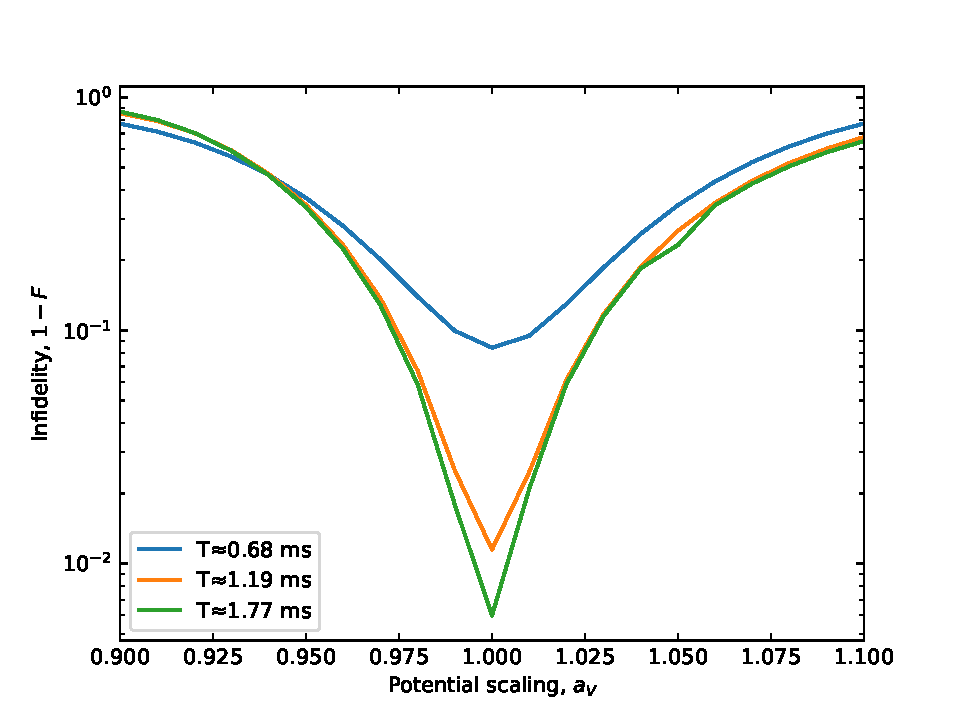
\includegraphics[width=\columnwidth]{graphics/newrobustness/robustness.pdf}
	\end{subfigure}
	\begin{subfigure}{\columnwidth}
		\centering
		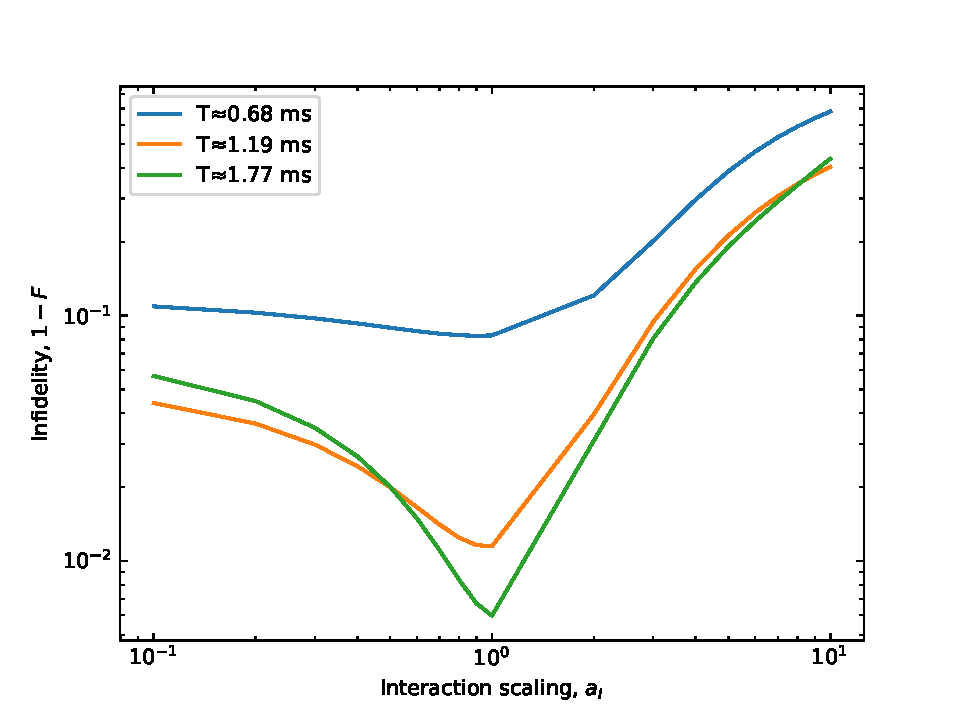
\includegraphics[width=\columnwidth]{graphics/newrobustness/interactionRobustness.pdf}
	\end{subfigure}
	\caption{Examining the robustness of an optimized solution wrt. scaling either the potential (top) or the atomic interaction (bottom).}
	\label{fig:robustness}
\end{figure}

As can be seen on figure \ref{fig:Clustering}, there are durations where the different control seeds reach similar levels of fidelity. This could indicate that they find the same or a similar optimized solution. The optimized solutions from figure \ref{fig:Clustering} with control duration $T\approx 0.685$ms are shown in figure \ref{fig:similarSolutions}. As can be seen on this figure, these optimized controls do not look alike despite reaching fidelity. It is most likely due to how different their initial control seeds are and so, one could argue that these seeds are located away from each other in the fidelity landscape. What should be noted though is the connection between seed frequency in $k\pi$ and the number of 'shakes' on the corresponding optimized control function. We see that for $k=2,3,4$ the number of shakes matches this frequency, which also strengthens the hypothesis for why these seeds don't converge to the same control. \\

\begin{figure}
	\begin{subfigure}{0.4\columnwidth}
		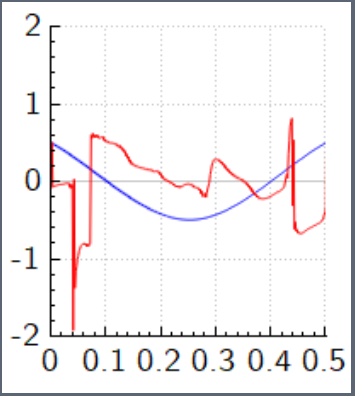
\includegraphics[width=\columnwidth]{graphics/similar_solutions/k2.PNG}
		\caption{$k=2$}
	\end{subfigure}
	\begin{subfigure}{0.4\columnwidth}
		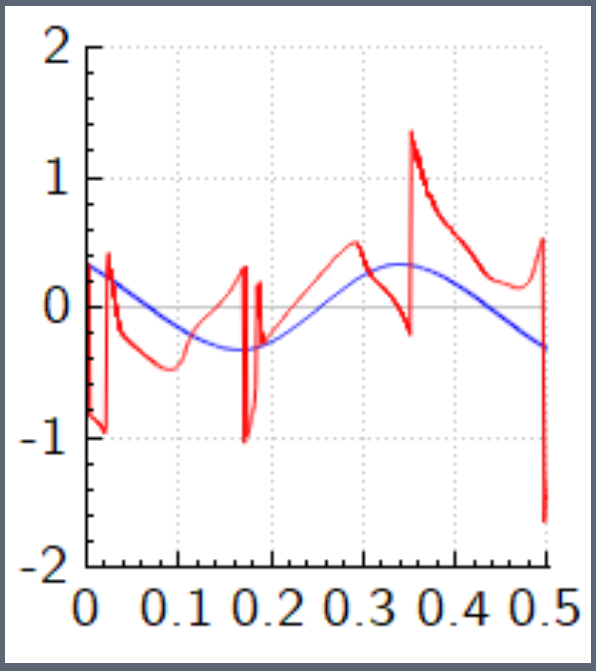
\includegraphics[width=\columnwidth]{graphics/similar_solutions/k3.PNG}
		\caption{$k=3$}
	\end{subfigure}
	\begin{subfigure}{0.4\columnwidth}
		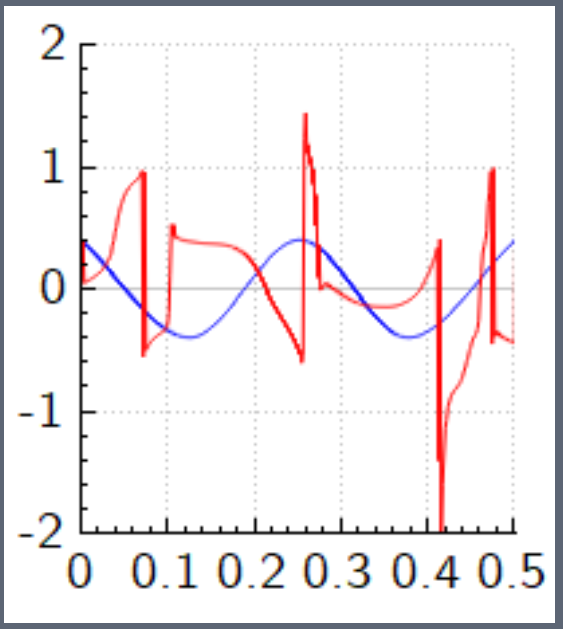
\includegraphics[width=\columnwidth]{graphics/similar_solutions/k4.PNG}
		\caption{$k=4$}
	\end{subfigure}
	\begin{subfigure}{0.4\columnwidth}
		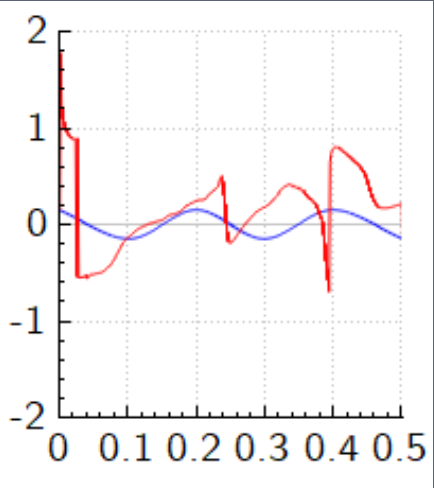
\includegraphics[width=\columnwidth]{graphics/similar_solutions/k5.PNG}
		\caption{$k=5$}
	\end{subfigure}
\caption{Screenshots from Quantum Composer showing \proc{Grape} optimized controls for the same seeds as in figure \ref{fig:Clustering}. First axis is time in scaling units, second axis is potential displacement from $x=0$ in scaling units. Each figure shows the control seed (blue) and \proc{Grape} optimized control (red) for that seed.}
\label{fig:similarSolutions}
\end{figure}

While examining the optimized solutions it was found that seeds with the same frequency in $k\pi$ would sometimes converge to similar optimized controls. Figure \ref{fig:SimilarTimescales} shows an example of this where the seed $A\cos(3\pi t/T)$ was optimized for different amplitudes $A$ and different durations $T$, yet still reached a very similar optimized solution. Notice also that both of these solutions have 2 shakes in the regime where it was found that optimal solutions were dominated by $\cos(2\pi t/T)$ frequencies \cite{QM2Paper}.

\begin{figure}
	\begin{subfigure}{0.4\columnwidth}
		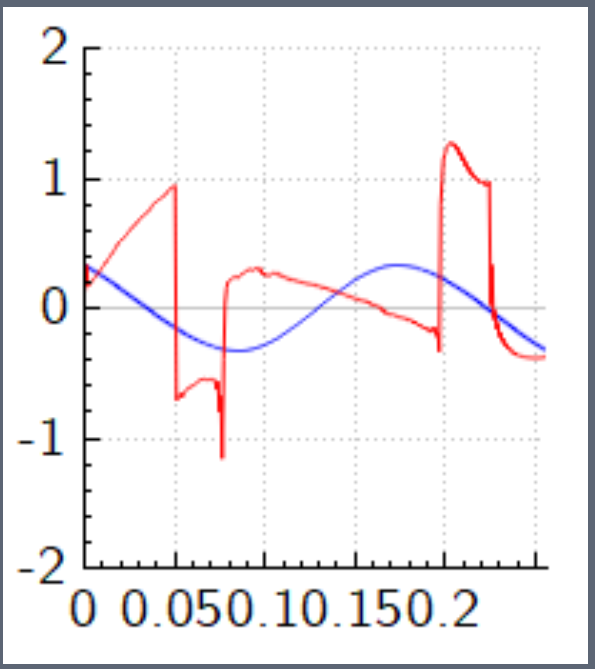
\includegraphics[width=\columnwidth]{graphics/similar_solutions/T02563k3A033.PNG}
	\end{subfigure}
	\begin{subfigure}{0.4\columnwidth}
		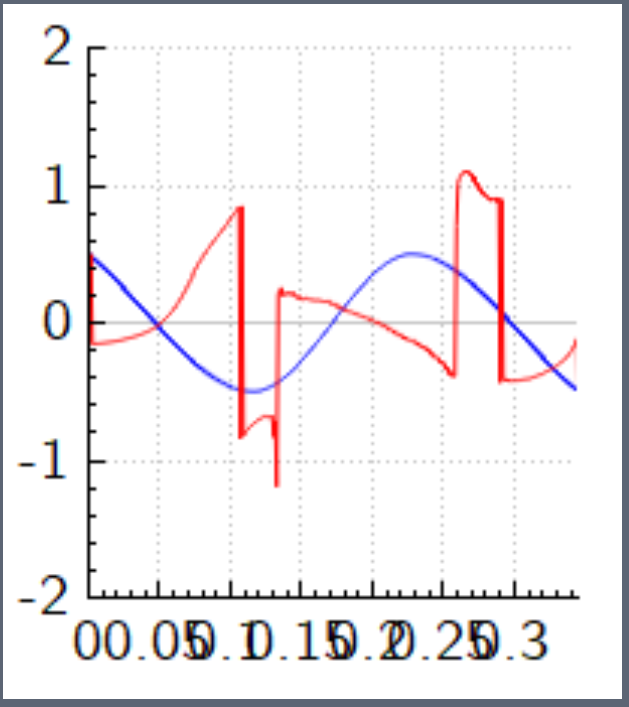
\includegraphics[width=\columnwidth]{graphics/similar_solutions/T03450k3A050.PNG}
	\end{subfigure}
	\caption{Screenshots of optimized controls of a similar seed for 2 different durations. The axis are read in the same way as in figure \ref{fig:similarSolutions}. Left: $T\approx 0.35$ms, $A=0.33$. Right: $T\approx 0.47$ms, $A=0.50$.}
	\label{fig:SimilarTimescales}
\end{figure}

\section{\label{sec:strats}Strategies}
% Function vs graph approach
Throughout working with this project, there has been two ways to determine the control function $u(t)$ in Composer: The control function is determined either by an analytical expression (using the Scalar expression node) or it is made by dragging the desired 'path' of displacement on a graph (using the Control node). These different nodes are shown in figure \ref{fig:Controls}. One can use both of these approaches when working with quantum control and they both have their advantages and disadvantages. \\

\begin{figure}[h]
	\begin{subfigure}[b]{0.4\columnwidth}
		\centering
		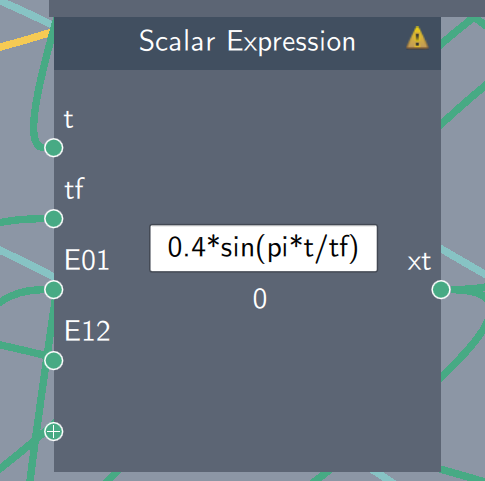
\includegraphics[width=\columnwidth]{graphics/ScalarExpressionNode.png}
		\caption{Scalar expression node}
	\end{subfigure}
	\hfill
	\begin{subfigure}[b]{0.45\columnwidth}
		\centering
		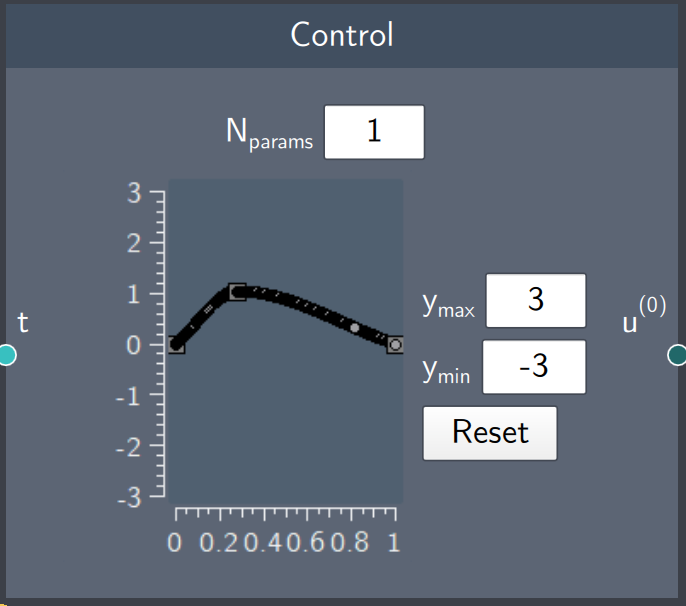
\includegraphics[width=\columnwidth]{graphics/ControlNode.png}
		\caption{Control graph node}
	\end{subfigure}
	\caption{Both nodes used for making a control function in Quantum Composer. The analytical function method (a) can take a number of input constants like final time $tf = T$, energy spacing between different states $(E01 = E_1 - E_0)$ and variables such as time $t$. The graph method (b) always scales the first axis such that the first point on the graph is at $t=t_0$ and the final point is at $t=T$.}
	\label{fig:Controls}
\end{figure}

% About function approach
Using an analytical expression as a control function, one gets the possibility of tweaking initial parameters to great accuracy such that the seed $\proc{Grape}$ gets already has a high fidelity. It is preferable to the graph approach in cases where a desired oscillation frequency is wanted e.g. the function $A\sin(E_{01}t)$. These kind of functions are difficult to mimic in the graph approach. When working with expressions independent of the final time $T$, adjusting this parameter translates into cutting the graph at different times. This is useful when exploring different functions and one finds that higher fidelity occurs at a different time than one currently works with. This method is shown in figure \ref{fig:funcAppr}. \\
\begin{figure}
	\def\svgwidth{\columnwidth}
	\input{graphics/functionAppr.pdf_tex}
	\caption{This figure shows how using an analytical control function can be used to reach a higher fidelity seed by altering the final time $T$. In this example we use the control function shown in red and the final time $T_1$. Evolving the system for a shorter(longer) time yields a higher fidelity though, and we can reach these fidelities by replacing the final time with $T_2$ ($T_3$). This method only works if the control function is independent of the final time.}
	\label{fig:funcAppr}
\end{figure}

% About graph approach
The Control graph node makes it possible to build up the control function as a series of steps. Here one can move one point on the graph and watch how the state evolves until that point, making it possible to optimize each step before going further. Since the graph node always spans the entire time interval $\{t_0,T\}$, this makes using the node useful when wanting to stretch or contract the entire function as shown on figure \ref{fig:graphAppr}. As demonstrated with the BEC in a harmonic potential in figure \ref{fig:HO}, there exists a complex relationship between $\beta$ and $T$ and so being able to keep the shape of the control function the same while altering the total time makes the node a beneficial tool to use.\\

\begin{figure}
	\def\svgwidth{\columnwidth}
	\input{graphics/graphAppr.pdf_tex}
	\caption{A visualization of one method that can be used to optimize fidelity when working with the graph node. If one tries to change the final time $T$ the resulting control function will be squeezed or stretched as a result. Altering the final time can be beneficial given the complex relationship between $\beta$ and $T$, but also as a tool to regulate the speed at which the potential moves. Using this approach also has the practical advantage that we can draw the graph such that $u(T)=0$ and so no matter the final time, the potential will always end up where it started. This is to be compared to the approach shown in figure \ref{fig:funcAppr} where this is not always the case and the state would possibly need to be transported back to its initial position.}
	\label{fig:graphAppr}
\end{figure}

When calculating the maximum reachable fidelity for some combination of $\beta$ and $T$ in the harmonic potential, the graph control node was used to create for $\proc{Grape}$. The overall strategy using this tool involved moving points on the graph into certain shapes and looking at how the initial (i.e. no $\proc{Grape}$) fidelity looked. I particularly liked the semi-circle shape of a $\sin(\pi t/T)$ function where the amplitude was varied. Another particular shape used in this work was generated by moving a single point around $0.1T$ or $0.9T$ to create a function which had a fast(slow) buildup to a maximum and then a slow(fast) return to the initial position. This wedge-like shape is shown on Fig. \ref{fig:Controls} (b).

Both of these strategies worked well and provided nice seeds for $\proc{Grape}$ to optimize on. Despite some cases where the fidelity changes significantly from small variations of $\beta$, the overall rule seems to be that something that works well for one value of $\beta$ will have a similar fidelity for nearby values of $\beta$ and so this was also used to find a good seed when $\beta$ was larger than $10$, since above this limit the system seemed a lot more sensitive to the initial control function with respect to reaching the highest possible fidelity for that particular combination of $\beta$ and $T$. \\

Measuring the Quantum Speed Limit for the quartic potential involved a combination of 2 strategies: The self-dubbed "up-to-down" and "down-to-up" approaches. \\

\proc{Up-to-down}:
\begin{enumerate}
	\item Pick $T_{up}$ to be a control duration estimated to lie above the QSL of the system
	\item Find an optimizable solution capable of reaching $F~0.99$
	\begin{itemize}
		\item If unable to do so, return to step 1. and choose a higher $T_{up}$
	\end{itemize}
	\item Gradually lower the duration in small steps, ensuring at each step that the control can still be optimized to $F~0.99$
	\begin{itemize}
		\item If the control is unable to reach $F~0.99$, one should try minor modifications to the control to see if this fixes it.
	\end{itemize}
	\item The lowest reachable $T$ is then the estimate of the QSL for the system. These steps can be repeated for another control function.
\end{enumerate}
The \proc{Up-to-down} procedure was my mainly used method for estimating the QSL of the system shown on Fig. \ref{fig:QSL}.\\

\proc{Down-to-up} works in a similar way to \proc{Up-to-down}, but in a reversed way:
\begin{enumerate}
	\item Pick $T_{down}$ such that it is estimated to lie below the QSL of the system.
	\item Try a number of different control functions and choose the most promising (i.e. the seed capable of reaching highest fidelity)
	\item $T$ is raised in small steps, at each step optimized and modified to check if $F~0.99$ is reachable
	\item The first time $F~0.99$ is reachable, the current $T$ is the estimated QSL for the system.
\end{enumerate}

%Cos vs Sin funcs
While reproducing the clustering of optimized controls data seen in Fig. \ref{fig:Clustering}, it became apparent that using cosine functions instead of sine functions could be advantageous for small timescales. One can use that fact that cosine is displaced from 0 at $t=0$ to ones advantage as it places the state on a steep slope of the potential. This generates motion of the state much faster than when initiating with a non-displaced control function. Similarly when the control is done, one can displace the potential such that the state feels rapid deceleration, thus reducing the velocity of the state much faster than if the control was constrained to end at $u(T)=0$. This behavior can also be seen on the optimized controls shown on Fig. \ref{fig:similarSolutions}, where both end points experience rapid displacement away from $x=0$. These advantages are similar to the "back-swing" solution for another problem described in \cite{QM2Paper}.
\section{\label{sec:disc}Discussion}
As explained in section \ref{subsec:strats}, the Quantum Composer software in this workshop allows for 2 different ways to construct control functions. While both methods have been used to explore the behavior of BECs subject to a controlled potential, the files only allow optimization of control functions made using the graph method.

While the graph method has its advantages as discussed above, the analytical function approach likewise has advantages that could be combined with $\proc{Grape}$. Having multiple approaches to the optimization problem would most likely be beneficial both from a perspective of understanding and from the perspective of being able to fine tune parameters for generating good seeds.\\

From what has been observed partially during exploring the dynamics of BECs and partially while gathering data for Fig. \ref{fig:HO} and the QSL in Fig. \ref{fig:QSL}, it is safe to say that when working with high values of $|\beta|$, the behavior of the system becomes difficult to predict. As final time goes up this only becomes more apparent, which was the conclusion that was reached after optimizing BECs in the harmonic potential.

This raises a (probably realistic) concern that the data shown in those 2 figures have been very sensitive to the initial conditions (i.e. the seed) and that other values could have been reached given more time to try different control functions. This is of course one of the problems with optimizing complex problems in the first place: They can be incredibly sensitive to initial conditions and while finding a local minimum is not a problem, finding the global one is a (very) difficult one.\\

Throughout both the exploration and data collection parts of this workshop, the control functions that have been used have for the most part been simple harmonic functions like $A\sin(\pi t/T)$ or other simple approaches such as the function seen in Fig. \ref{fig:Controls} (b).

However, what has also become apparent while working with $\proc{Grape}$ is that it usually introduces(after a number of iterations) rapidly oscillating behavior on parts of the graph. It is understood that this is most likely due to the way $\proc{Grape}$ optimizes control functions, but it also shows that more complex control functions are not necessarily bad and can actually in some cases reach much higher fidelity than their 'simpler' counterparts. In any case the simpler control functions seem like a good way to explore the fidelity landscape (so-called "global search") while optimization algorithms such as \proc{Grape} are then used to find the locally optimal control, usually more complex than the input seed. \\

As described in section \ref{subsec:numericalLimitations}, some of the ways to explore this problem are blocked by numerical instabilities. What has not yet been tested is how changing the discretized space or discretized timescale (i.e. by adding more points and/or having a larger space) could potentially solve some of these problems. What has been found though, is that changing these parameters also introduce much higher variance to either ground or 1st excited state and so do not currently seem like viable strategy for solving this numerical problem, although it cannot be excluded either.


\section{\label{sec:conclusion}Conclusion}
It has been demonstrated that the behavior of BECs are sensitive to the parameters $\beta$ and $T$. As it has been shown in Fig. \ref{fig:HO}, this changed behavior compared to a single particle can be beneficial and capable of reaching higher fidelity than is otherwise possible. On the other hand it is also apparent that $\beta$ introduces an unpredictability into the system as well as numerical inaccuracy of the Hamiltonian eigenstates. It has also been shown that the $\beta$ term in \eqref{eq:Hbec} increases the QSL up to a estimated value of 2 times that of a single particle for the case $\beta=25$. It was also attempted to cluster the performance of $\cos(k\pi t/T)$ control seeds to the frequency $k$, although the data shown in Fig. \ref{fig:Clustering} shown that the seed frequency and optimized performance are not connected in a straightforward manner. What seems more promising is analyzing the number shakes in the optimized solutions and clustering these. The robustness of some optimized solutions have been explored both regarding a scaled potential and a scaled atomic interaction, as is shown in Fig. \ref{fig:robustness}.

Some strategies involving choosing a control function have also been explored. The differences, advantages and disadvantages of using either an analytical function node or a graph node to determine the control function have been discussed. This includes how varying $T$ affects the control function, as has been illustrated on figures \ref{fig:funcAppr} and \ref{fig:graphAppr}. Finally, 2 concrete strategies for determining the QSL in this problem have been explained, both using the graph node to create a control function.

Numerical boundaries of the software used have been demonstrated and their implications for exploring the challenge have been discussed.

Future aspects of this problem that could be interesting to research include:
\begin{itemize}
	\item Increasing the resolution of Fig. \ref{fig:QSL}, since it has been shown that $\beta=-10$ is the optimizable limit for this problem.
	\item Analyze the optimized controls from Fig. \ref{fig:Clustering} to make a new $(T,F)$ plot where each point is colorcoded based on the number of shakes in its optimized solution. It is expected that this will replicate what was found in \cite{QM2Paper}.
	\item Compare the robustness of optimized solutions with different number of 'shakes', but where both solutions reach similar fidelities.
\end{itemize}

% Create the reference section using BibTeX:
% comment the line below if you do not have a bibliography
\bibliography{thebibliography}

\end{document}
